% Produktdarstellung.tex
\subsection{Produktdarstellung}
Eine zentrale Komponenten der Anwendung ist die Darstellung einer Produktseite, welche auf dem \textit{SVG}-Format basiert.
Das SVG-Format ist eine XML-basiertes Markup-Sprache welche eine zweidimensionale Grafik beschreibt und innherhalb von HTML-Quelltext platziert werden kann \autocite[vgl.][]{AboutSVG}. 

Wie von Abbildung \ref{fig:Produktdarstellung} zu entnehmen ist, werden für das Erzeugen der \textit{SVG}-Struktur \textit{ReactJS}-Komponenten genutzt, die exklusiv für die Produktdarstellung erstellt wurden. Diese Komponenten finden in keinem anderem Zusammenhang Verwendung und sind eng an die Produktdarstellung gekoppelt. 
Zur Darstellung des Produktes gehören das Darstellen von Beschnittlinien, Falzlinien, Nutlinien, Bereichen die nicht bedruckbar sind, sowie Seitenbezeichnungen. Bei einigen Produkten, Textilien oder Werbeprodukte, kann im Hintergrund eine Abbildung des Produktes dargestellt werden. Die Komponente \textit{SVGPageRenderer} ist für verantwortlich für die Produktdarstellung und wird Komponente \textit{PagePresenter.tsx} eingesetzt. Diese wiederum ist für Präsentation des Produktes innerhalb des FreeDesign-Editors verantwortlich und ermöglicht das Rotieren, Skalieren sowie das Verschieben der Darstellung. 


Das Produkt wird durch eine Struktur beschrieben, welche im \textit{core}-Ordner hinterlegt ist. Die Struktur enthält sowohl geometrische Information für die Produktdarstellung, als auch Produktspezifische eigenschaften, wie die Existenz von Beschnittlinien. 

\begin{figure}[H]
    \centering
    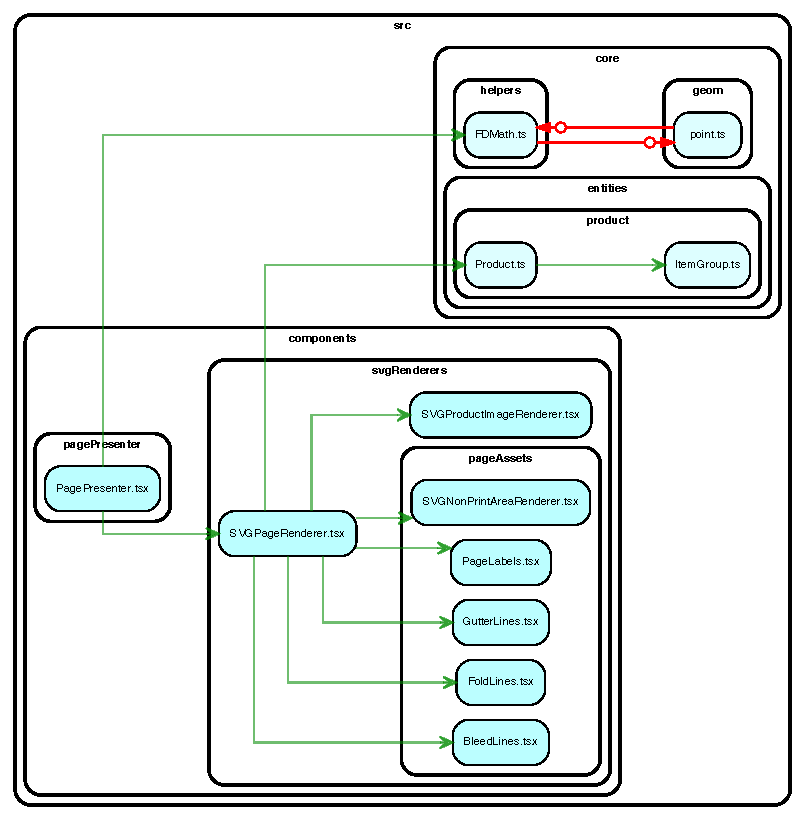
\includegraphics{diagrams/Ist-Architektur/page-presenter-analysis.pdf}
    \caption{Abhängigkeiten der Komponenten für Produktdarstellung}
    \label{fig:Produktdarstellung}
\end{figure}
 
Für die Darstellung innerhalb des FreeDesign-Editors ist die Nutzung von mathematischen Operationen notwendig, die im Anwendungskern definiert sind. 

Damit stellt sich die Darstellung einer Produktseite als sehr klar strukturiert dar. 